\chapter{Đọc thêm: Thanh khoản và tác động của cú sốc thông tin (Chương 3)}
\label{ch:M1L2-reading}

\section{Thanh khoản và tác động của các cú sốc thông tin: Ứng dụng trong khóa học Kinh tế Vĩ mô}

Mối quan hệ giữa kinh tế vĩ mô và giá cổ phiếu là cực kỳ quan trọng. Vậy nếu điều đó đúng, thì nền kinh tế ảnh hưởng đến giá cổ phiếu như thế nào và ngược lại? Trong nhiều trường hợp, đó là tin tức về kinh tế vĩ mô và chính xác hơn là tin tức bất ngờ. Việc công bố những tin tức "bất ngờ" về nền kinh tế được gọi là "cú sốc thông tin" (information shocks), thứ có thể có tác động nhanh chóng và đáng kể đến giá cổ phiếu. Các cú sốc thông tin về cơ bản khác với "cú sốc thanh khoản" (liquidity shocks) đã được mô tả trước đó trong chương Tài chính. Trong trường hợp của các cú sốc thanh khoản, chúng ta đã thấy cấu trúc của chính thị trường tài chính cùng với số lượng và chất lượng của các lệnh được gửi có thể ảnh hưởng như thế nào đến khả năng của các nhà đầu tư trong việc tìm ra giá "thực" của một cổ phiếu thông qua quá trình được gọi là "khám phá giá" (price discovery). Trong trường hợp của chúng ta ở đây, các cú sốc thông tin cũng có tác động lớn đến quá trình khám phá giá, nhưng động lực chính của những cú sốc này là sự xuất hiện của những tin tức bất ngờ, chứ không phải do thiếu thanh khoản trong một thị trường tài chính.\footnote{Như đã thảo luận trong chương Tài chính, các thị trường tài chính có thể đạt được "hiệu quả thông tin" nếu chúng xử lý và kết hợp các tin tức bất ngờ một cách nhanh chóng và chính xác vào giá cổ phiếu hiện tại. Theo "giả thuyết thị trường hiệu quả" (EMH), nếu thị trường nhanh chóng và chính xác phản ánh thông tin mới vào giá cổ phiếu, thì hành vi của các mức giá này sẽ giống như một "bước đi ngẫu nhiên" (random walk) và do đó dẫn đến những biến động giá không thể đoán trước theo thời gian. Như đã lưu ý trong chương Tài chính, các thị trường tài chính tương đối hiệu quả nhưng không phải lúc nào cũng hoàn hảo, và do đó có thể mang lại cơ hội cho những nhà đầu tư và nhà giao dịch nhanh nhạy phát hiện ra các xu hướng giá trước khi những người khác khám phá ra.}

Trong chương này, chúng tôi mô tả một số ví dụ về các cú sốc liên quan đến kinh tế vĩ mô và tác động của chúng đối với thị trường chứng khoán Hoa Kỳ, cũng như các mối quan hệ tương hỗ giữa thị trường tài chính và nền kinh tế.

Với quy mô khổng lồ và sự phức tạp của nền kinh tế quốc gia, thông tin liên quan đến kinh tế vĩ mô bao gồm rất nhiều yếu tố. Vậy yếu tố nào là quan trọng nhất? Đầu tiên và quan trọng nhất là lãi suất, thứ áp dụng cho từng công ty cá biệt, các ngành cụ thể, cũng như các lĩnh vực rộng lớn hơn của nền kinh tế. Trong kinh tế vĩ mô, mối quan hệ chủ yếu tập trung vào sự tương tác giữa lãi suất, khu vực tư nhân (bao gồm người tiêu dùng, nhà đầu tư và doanh nghiệp) và các nhà hoạch định chính sách của chính phủ tại Cục Dự trữ Liên bang (thông qua chính sách tiền tệ) và Bộ Tài chính Hoa Kỳ (thông qua chính sách tài khóa). Do lãi suất đại diện cho giá thuê vốn (rental price of money), nên chúng đóng vai trò là cầu nối chính giữa "thế giới thực" của kinh tế vĩ mô và "thế giới tài chính" của thị trường cổ phiếu và trái phiếu. Cả khu vực tư nhân và chính phủ đều theo dõi sát sao lãi suất như một tín hiệu về tình trạng hiện tại và tương lai của nền kinh tế nhằm đưa ra các quyết định phân bổ nguồn lực khan hiếm vào những mục đích sử dụng hiệu quả nhất. Thông qua thanh khoản do thị trường tài chính cung cấp, các nhà đầu tư có thể chuyển các khoản tiết kiệm của mình vào những khoản đầu tư sinh lời, điều này cuối cùng dẫn đến tăng trưởng kinh tế mạnh mẽ hơn cho xã hội. Do đó, các nhà kinh tế học và nhà đầu tư nên xem xét thanh khoản của thị trường tài chính để hiểu rõ hơn về cách thế giới tài chính và thế giới thực tương tác với nhau.

\subsection{Điều kiện kinh tế, Chu kỳ kinh doanh và Vai trò của Lãi suất}

Động lực chính của những biến động chu kỳ kinh doanh ở hầu hết các quốc gia là đầu tư của doanh nghiệp, và những thay đổi đột ngột trong đầu tư này có thể dẫn đến bùng nổ kinh tế cũng như suy thoái. Do đó, các giám đốc điều hành kinh doanh liên tục đánh giá bối cảnh kinh tế để xem người tiêu dùng đang mua gì (và với số lượng bao nhiêu), cũng như theo dõi niềm tin của người tiêu dùng để quyết định mức độ đầu tư cho tương lai. Khi nhu cầu của người tiêu dùng tăng và giảm, các doanh nghiệp phản ứng nhanh chóng bằng cách điều chỉnh số lượng đầu tư vào nhà máy, thiết bị, hàng tồn kho, nghiên cứu và công nghệ mới. Những điều chỉnh này có thể dẫn đến những thay đổi mạnh mẽ về việc làm và tiền lương, từ đó tác động đến những thay đổi tiếp theo trong mô hình chi tiêu của người tiêu dùng. Mối quan hệ giữa đầu tư và tiêu dùng là mang tính tuần hoàn, và điều này dẫn đến tính chất chu kỳ của hầu hết các nền kinh tế, khi các đợt bùng nổ được theo sau bởi các cuộc suy thoái, cuối cùng dẫn đến sự phục hồi và sau đó là các đợt bùng nổ kinh tế tiếp theo.

Lãi suất cũng bị ảnh hưởng lớn bởi đầu tư của doanh nghiệp vì các công ty thường vay tiền từ những người cho vay và các nhà đầu tư để tài trợ cho việc mở rộng trong tương lai. Nhu cầu tiền mặt gia tăng này tạo áp lực làm tăng lãi suất trừ khi ngân hàng trung ương của một quốc gia, chẳng hạn như Cục Dự trữ Liên bang Hoa Kỳ (thường được gọi là "Fed"), tăng cung tiền.

Sự tương tác giữa đầu tư và lãi suất rất phức tạp vì các tác động có thể diễn ra đồng thời về bản chất. Cụ thể, đầu tư kinh doanh không chỉ ảnh hưởng đến lãi suất, mà mức lãi suất, đến lượt nó, lại ảnh hưởng đến mức độ đầu tư. Ví dụ, nếu người tiêu dùng đột nhiên mua nhiều hàng hóa và dịch vụ hơn, các doanh nghiệp sẽ đầu tư nhiều hơn và cuối cùng sẽ đẩy lãi suất lên do nhu cầu tiền mặt tăng. Tuy nhiên, nếu lãi suất tăng quá cao, các doanh nghiệp sẽ cắt giảm đầu tư vì chi phí tài trợ cho nhà máy, thiết bị mới hoặc hàng tồn kho lúc này có thể vượt quá lợi nhuận mà doanh nghiệp có thể kiếm được từ khoản đầu tư mới này. Cuối cùng, việc giảm đầu tư do lãi suất cao hơn sẽ dẫn đến nhu cầu tiền mặt thấp hơn. Điều này sau đó sẽ khiến lãi suất giảm trong tương lai, từ đó tạo ra một chu kỳ kinh điển giữa đầu tư và lãi suất.

Do đó, những thay đổi trong đầu tư kinh doanh được theo dõi sát sao bởi các nhà hoạch định chính sách, chẳng hạn như những người tại Cục Dự trữ Liên bang. Fed sẽ cố gắng kích thích và ổn định nền kinh tế bằng cách điều chỉnh lãi suất Quỹ Liên bang (Federal Funds rate)\footnote{Lãi suất Quỹ Liên bang là mức lãi suất mà các ngân hàng thương mại tính cho nhau khi vay qua đêm để đáp ứng nhu cầu thanh khoản ngắn hạn.} nhằm duy trì sự tăng trưởng ổn định với lạm phát thấp. Để điều chỉnh mức lãi suất chủ chốt này lên (hoặc xuống), Fed thường sử dụng các nghiệp vụ thị trường mở ("OMO") để bán (hoặc mua) chứng khoán Kho bạc Hoa Kỳ (U.S. Treasury securities) trên các thị trường trái phiếu chính phủ, nơi các đối tác giao dịch chính là các tổ chức tài chính như ngân hàng thương mại và các nhà môi giới chứng khoán (broker-dealers). Khi Fed bán Trái phiếu Kho bạc qua các hoạt động OMO, mục tiêu là giảm cung tiền và tăng lãi suất Quỹ Liên bang (giả sử nhu cầu tiền mặt vẫn tương đối ổn định). Bằng cách bán Trái phiếu Kho bạc, Fed đang rút đô la khỏi nền kinh tế và làm giảm cung tiền do các nhà đầu tư phải từ bỏ tiền mặt của họ để mua các chứng khoán chính phủ này. Các nhà kinh tế gọi đây là chính sách tiền tệ "thắt chặt" (contractionary monetary policy) bởi vì mục tiêu của việc tăng mức lãi suất then chốt này là khiến các ngân hàng và những người cho vay khác tăng lãi suất cho vay của họ, và qua đó, làm cho các doanh nghiệp và người tiêu dùng phải chịu chi phí cao hơn để chi trả cho các khoản đầu tư và tiêu dùng bổ sung. Điều này cuối cùng có thể dẫn đến sự thu hẹp của nền kinh tế thông qua việc giảm đầu tư của doanh nghiệp, vì lãi suất cao hơn có thể "làm nguội" một nền kinh tế đang trên đà "quá nóng" do lạm phát giá cả gia tăng. Ngược lại, một chính sách tiền tệ "mở rộng" (expansionary monetary policy) xảy ra khi Fed mua Trái phiếu Kho bạc để bơm thêm tiền vào nền kinh tế nhằm giảm lãi suất Quỹ Liên bang và kích thích đầu tư từ các doanh nghiệp và người tiêu dùng.

\subsection{Cục Dự trữ Liên bang và Mối liên kết giữa Kinh tế vĩ mô và Thị trường Tài chính}

Hoạt động OMO của Fed tạo ra một "vòng phản hồi tương tác" (interactive feedback loop) liên tục giữa nền kinh tế vĩ mô và thị trường tài chính. Khi các điều kiện kinh tế vĩ mô và lãi suất thay đổi, cả Fed và các thành viên tham gia thị trường như ngân hàng, nhà môi giới và nhà quản lý tài sản đều điều chỉnh danh mục nắm giữ của họ, không chỉ đối với chứng khoán Kho bạc Hoa Kỳ mà còn đối với các tài sản rủi ro hơn như trái phiếu doanh nghiệp và cổ phiếu vốn cổ phần. Các nhà đầu tư trên thị trường tài chính phản ứng với những tin tức bất ngờ về nền kinh tế và lãi suất vì giá trị của một cổ phiếu hay trái phiếu được xác định bởi giá trị hiện tại của các dòng tiền mặt dự kiến trong tương lai của nó. Như đã lưu ý trong chương Vi mô, phản ứng này của nhà đầu tư bị thúc đẩy bởi những thay đổi trong lãi suất phi rủi ro, điều này có thể ảnh hưởng đến Đường Thị trường Vốn (Capital Market Line) theo Mô hình Định giá Tài sản Vốn (CAPM). Trong mô hình đó, khi lãi suất phi rủi ro tăng lên, điểm giao cắt (intercept) tăng lên, độ dốc (slope) giảm xuống và điểm tiếp tuyến (tangency) với đường biên hiệu quả (efficient frontier) di chuyển lên trên và sang phải, qua đó làm tăng tỷ suất sinh lợi yêu cầu của các nhà đầu tư đối với danh mục thị trường. Khái niệm Đường Thị trường Vốn giúp giải thích cách thức các hành động và tuyên bố chính sách của Fed có thể tạo ra các cú sốc thông tin, dẫn đến lượng lớn hoạt động giao dịch trong tất cả các loại chứng khoán, điều này ngược lại, phụ thuộc vào thanh khoản của các thị trường tài chính. Thông qua việc giao dịch hàng nghìn tỷ đô la chứng khoán hằng ngày này, các thị trường tài chính phục vụ một mục đích quan trọng là cơ chế chính để khám phá ra mức giá phù hợp cho các tài sản tài chính. Như đã lưu ý trước đó trong các chương Tài chính và Vi mô, khám phá giá là một chức năng chính của bất kỳ thị trường tài chính hoạt động trơn tru nào.

Một ví dụ điển hình về vòng phản hồi tương tác này có thể thấy trong thông báo tháng 10 năm 2018 của Fed về kế hoạch tiếp tục tăng lãi suất và cách chính sách thắt chặt này đã gây sốc cho các thị trường chứng khoán Hoa Kỳ, khiến giá giảm mạnh vào cuối tháng 12 năm 2018. Để phản ứng với phản ứng tiêu cực này của thị trường, chủ tịch Fed, Jerome Powell, đã tuyên bố vào đầu tháng 1 năm 2019 rằng quan điểm thắt chặt của Fed sẽ được "tạm dừng". Các thị trường tài chính coi đây là tin tốt vì lo ngại rằng việc tiếp tục tăng lãi suất Quỹ Liên bang có thể khiến nền kinh tế Hoa Kỳ rơi vào suy thoái. Thị trường chứng khoán Hoa Kỳ đã phản ứng rất tích cực với sự thay đổi trong chính sách tiền tệ này trong quý đầu tiên của năm 2019. Thấy được điều này, Fed cuối cùng đã quyết định cắt giảm lãi suất ba lần, dẫn đến sự gia tăng 29\% của chỉ số S\&P 500 trong năm 2019. Thêm chi tiết về ví dụ này về sự tương tác giữa nền kinh tế và thị trường tài chính sẽ được thảo luận ở phần sau của chương này.

\subsection{Tác động của Cú sốc Thông tin đối với Kỳ vọng Phân kỳ và Khám phá Giá}

Những thay đổi trong chính sách của Fed có thể ảnh hưởng đến thanh khoản của thị trường tài chính không chỉ trực tiếp bằng hoạt động OMO của Fed mà còn thông qua các "tín hiệu" thông tin ẩn chứa trong những thay đổi chính sách này. Ví dụ, một đợt cắt giảm bất ngờ lãi suất Quỹ Liên bang là một cú sốc thông tin có thể ra tín hiệu cho các nhà đầu tư và giám đốc điều hành doanh nghiệp rằng nền kinh tế hiện đang yếu, nhưng đồng thời, nó cũng cho mọi người biết rằng Fed đang hành động để kích thích các điều kiện kinh tế và do đó sẽ củng cố kinh tế vĩ mô trong tương lai. Điều này có thể tạo ra "kỳ vọng phân kỳ" (divergent expectations - một khái niệm được thảo luận trong chương Tài chính), nơi một số thành viên tương đối bi quan của thị trường sẽ giao dịch dựa trên sự suy yếu kinh tế ngắn hạn (ví dụ: bằng cách mua trái phiếu khiến giá trị của chúng tăng lên và lãi suất giảm, đồng thời cũng bán cổ phiếu). Ngược lại, các thành viên lạc quan hơn sẽ tập trung vào những triển vọng tích cực của một nền kinh tế vững mạnh trong dài hạn hơn và chọn đầu tư vào các tài sản rủi ro có khả năng sinh lời tốt trong một nền kinh tế mở rộng (ví dụ: bằng cách bán trái phiếu và mua cổ phiếu).

Trong thuật ngữ của thị trường tài chính, các nhà giao dịch bi quan thường được gọi là "những con gấu" (bears), trong khi các nhà giao dịch lạc quan được miêu tả là "những con bò tót" (bulls). Giao dịch trên các thị trường tài chính giữa hai loại nhà đầu tư này sau đó sẽ giúp khám phá ra mức giá "cân bằng" (equilibrium) thích hợp của cổ phiếu và trái phiếu. Các mức giá này là những tín hiệu mang tính thông tin. Tuy nhiên, không chỉ mất cả một ngày giao dịch mà còn có thể mất vài ngày (hoặc thậm chí vài tuần) để những con bò tót và những con gấu giao dịch với nhau cho đến khi một mức giá cân bằng mới được khám phá. Quá trình khám phá giá kéo dài này xảy ra vì các báo cáo kinh tế được công bố sau cú sốc thông tin ban đầu đôi khi có thể mâu thuẫn về bản chất. Ví dụ, dữ liệu kinh tế theo chiều hướng giá lên (bullish) được công bố vào một ngày có thể được theo sau bởi dữ liệu giá xuống (bearish) vào ngày hôm sau, do đó gieo rắc sự nhầm lẫn về tác động thực sự của các báo cáo này đối với giá của một cổ phiếu.

Để minh họa cho vai trò quan trọng của việc khám phá giá, chúng ta có thể sử dụng một ví dụ được đơn giản hóa dựa trên giá cổ phiếu của một công ty giả định, ABC. Các nghiên cứu học thuật trước đây của Handa, Schwartz và Tiwari (2003) gợi ý rằng chúng ta có thể mô tả sự phân kỳ trong kỳ vọng của các nhà đầu tư bằng cách chia một nhóm người tham gia thành hai nhóm. Hãy gọi một nhóm là "bò tót" và nhóm kia là "gấu". Chúng ta có thể giả định rằng phe bò định giá cổ phiếu ABC ở mức 30 đô la và phe gấu định giá cổ phiếu ABC ở mức 20 đô la. Phe bò là những người mua, và phe gấu là những người bán do sự phân kỳ kỳ vọng về giá trị tương lai của cổ phiếu dựa trên một số tin tức kinh tế vĩ mô bất ngờ như sự thay đổi đột ngột trong chính sách tiền tệ của Cục Dự trữ Liên bang. Giả sử những người tham gia lần lượt đến thị trường tài chính và (1) đăng các lệnh mua hoặc bán hoặc (2) giao dịch ngay lập tức ở mức giá mua hoặc giá chào bán được thiết lập bởi các lệnh đã được đặt trước đó. 

Giá mua và giá chào bán cân bằng cho cổ phiếu ABC có thể được xác định nếu biết thêm một thông tin nữa - tỷ lệ phần trăm những người tham gia là phe bò (ký hiệu là k) và tỷ lệ phần trăm những người tham gia là phe gấu (ký hiệu là $1-k$). Trong bối cảnh được đơn giản hóa này, sự phân kỳ trong kỳ vọng giữa các bên tham gia có hai chiều hướng: (1) độ lớn của chênh lệch giữa các mức định giá cao và thấp (trong trường hợp của chúng ta là $\$30-\$20$) và (2) sự phân bổ của các nhà đầu tư giữa hai định giá (như được thể hiện bởi k). Do đó, giá trị của cổ phiếu ABC sẽ nằm đâu đó trong khoảng từ 20 đô la đến 30 đô la tùy thuộc vào giá trị của k. Ví dụ, nếu một nửa số nhà giao dịch là theo chiều hướng giá lên ($k=.50$), thì giá cân bằng sẽ là 25 đô la (tức là $.50\times\$30$ cộng với $.50\times\$20=\$25$).

Làm thế nào những người tham gia biết hoặc tìm ra giá trị của k? Cách chính là quan sát các lệnh được gửi đến thị trường tài chính. Những lệnh này được tạo ra để phản ứng với tin tức về triển vọng của ABC cũng như các điều kiện kinh tế vĩ mô nói chung. Vì vậy, những người tham gia khám phá ra giá trị của k thông qua các lệnh được tiết lộ trong quá trình giao dịch diễn ra. Khi các giao dịch này được báo cáo cho mọi người nhìn thấy, giá cổ phiếu ABC sẽ biến động để phản ứng với những niềm tin thay đổi về k.

Trong các thị trường thực tế, kỳ vọng phân kỳ của người tham gia được phân bổ trên một phạm vi định giá rộng hơn, và chúng ta không thể chỉ tham chiếu đến một biến k. Tuy nhiên, kết luận vẫn đúng - khi kỳ vọng có sự phân kỳ, giá phải được khám phá thông qua quá trình giao dịch trên các thị trường tài chính. Quá trình này không hề đơn giản và đôi khi có thể lộn xộn, kéo dài khi các nhà đầu tư phải sàng lọc vô số tín hiệu từ cả thị trường tài chính và kinh tế vĩ mô, nhiều trong số đó có thể mâu thuẫn nhau.

\subsection{Các Loại Hình Thị trường Tài chính Khác nhau}

Như đã thảo luận trong ví dụ về sổ lệnh giới hạn của chương Tài chính, một thị trường tài chính mỏng (thin), thanh khoản kém sẽ áp đặt chi phí giao dịch cao hơn cho các nhà đầu tư và có thể ngăn cản một số người tham gia đặt lệnh ngay từ đầu. Ví dụ, trong một thị trường dựa trên sổ lệnh giới hạn (limit order book) thanh khoản kém (còn được gọi là thị trường "điều khiển bằng lệnh" (order-driven) liên tục), một cú sốc thông tin có thể gây ra sự gia tăng đột ngột các lệnh mua hoặc bán, và điều này có thể dẫn đến mức chênh lệch giá chào mua-chào bán (bid-ask spread) rộng hơn. Nếu không có các mức giá chào mua và chào bán mới được đưa vào sổ lệnh giới hạn, mức chênh lệch bid-ask mà các nhà đầu tư phải trả sẽ cao hơn rất nhiều, và do đó, việc giao dịch cổ phiếu của công ty sẽ trở nên đắt đỏ hơn. Ngoài ra, mức chênh lệch cao hơn này có thể dẫn đến sự biến động giá lớn hơn, bởi vì ngay cả khi báo giá mua và báo giá bán tốt nhất vẫn không đổi, giá giao dịch sẽ bật lên bật xuống giữa mức giá chào mua và mức giá chào bán do sự xuất hiện gián đoạn của các lệnh thị trường (market orders) muốn bán khớp với mức giá chào mua thấp hơn, và các lệnh thị trường muốn mua khớp với mức giá chào bán cao hơn nhiều. Tác động này thường được gọi là "bid-ask bounce" (sự nảy lên nảy xuống giữa giá mua và giá bán), và sự nảy này góp phần tạo ra biến động giá trong ngắn hạn.

Giá cổ phiếu cũng trở nên biến động hơn trong một sổ lệnh mỏng (thin order book) do "tác động thị trường" (market impact), xảy ra khi một lệnh mua lớn đẩy giá khớp lệnh lên cao hơn mức giá chào bán tốt nhất, hoặc một lệnh bán lớn đẩy giá xuống thấp hơn mức giá chào mua tốt nhất. Khi tác động thị trường lớn, sự biến động giá sẽ tăng lên do giá thường sẽ quay trở lại (revert) các mức quan sát được ngay trước khi lệnh thị trường lớn đó được đặt. Quá trình khám phá giá cũng có thể trở nên khó khăn hơn trong một thị trường mỏng, và nếu đúng như vậy, điều này cũng sẽ góp phần làm tăng biến động giá.

Hệ quả là, một sổ lệnh mỏng có thể làm cho quá trình khám phá giá khó khăn hơn, từ đó dẫn đến những tín hiệu kém tính thông tin hơn về cách các nhà đầu tư đang phản ứng với những tin tức liên quan đến kinh tế vĩ mô và sức khỏe tài chính của một cổ phiếu cụ thể như ABC. Do đó, các tín hiệu từ một thị trường tài chính kém thanh khoản sẽ "nhiễu" (noisier) hơn so với những tín hiệu được tạo ra bởi một thị trường sâu (deep), có tính thanh khoản cao. Trong trường hợp cực đoan, một thị trường tài chính rất kém thanh khoản bị giáng đòn bởi các cú sốc thông tin thường xuyên sẽ dẫn đến những tín hiệu không đáng tin cậy từ các nhà đầu tư, và vòng phản hồi tương tác giữa kinh tế vĩ mô và thị trường tài chính sẽ bị phá vỡ. Kết quả này là tiêu cực đối với tất cả các bên vì các nhà đầu tư, giám đốc điều hành doanh nghiệp và các nhà hoạch định chính sách không còn có được dòng thông tin tự do luân chuyển về cách hành động của họ đang ảnh hưởng đến cả nền kinh tế vĩ mô và thị trường tài chính. Kết quả là, thanh khoản kém có thể cản trở tăng trưởng kinh tế và làm xói mòn lợi nhuận do cổ phiếu và trái phiếu mang lại.

Bên cạnh cấu trúc sổ lệnh giới hạn, hay cấu trúc thị trường điều khiển bằng lệnh liên tục được mô tả trong chương Tài chính, có hai cách chính khác để tổ chức một thị trường tài chính: (1) đấu giá định kỳ (periodic call auction) và (2) thị trường có sự tham gia của nhà tạo lập thị trường (dealer market - hay còn gọi là thị trường "điều khiển bằng báo giá" (quote-driven)). Phiên đấu giá định kỳ là một thị trường điều khiển bằng lệnh định kỳ (ngược lại với liên tục). Các cấu trúc thị trường thay thế này có thể giúp ích cho những người mua và người bán lớn, những người mà nếu không có các cấu trúc này, có thể sẽ ngần ngại khi đưa lệnh của họ vào một thị trường liên tục điều khiển bằng báo giá. Những nhà giao dịch này e ngại việc nộp các lệnh lớn vì sợ đẩy giá lên hoặc xuống một cách không chính đáng (được gọi là tác động thị trường). Một mối quan ngại khác đối với những người mua/người bán lớn này là việc các nhà giao dịch khác có thể phát hiện ra lệnh của họ, điều này có thể dẫn đến việc giao dịch ở mức giá không thuận lợi (thường được gọi là "rò rỉ thông tin" (information leakage)). Các lệnh không được tiết lộ được gọi là "thanh khoản ngầm" (latent liquidity).

Như đã thảo luận trong chương Tài chính, trong một phiên đấu giá định kỳ (call auction), các lệnh của người tham gia được gom lại cùng nhau để thực hiện đồng thời tại một mức giá thanh toán (clearing price) duy nhất vào một thời điểm đã được thông báo trước. Khi thị trường được gọi (called), tất cả các lệnh mua bằng hoặc lớn hơn mức giá thanh toán đều có thể được thực thi, tương tự như tất cả các lệnh bán bằng hoặc thấp hơn mức giá thanh toán. Các mức giá giao dịch được thiết lập ở những giá trị tối đa hóa số lượng cổ phiếu được khớp lệnh. Bằng cách gom (batching) nhiều giao dịch lại cùng nhau, một phiên đấu giá định kỳ sẽ tập trung được thanh khoản và qua đó, có thể làm giảm đáng kể chi phí giao dịch cho người tham gia. Các phiên đấu giá này cũng tạo điều kiện thuận lợi cho quá trình "khám phá số lượng" (quantity discovery) bằng cách cho phép các lệnh lớn hơn được thực thi với ít tác động thị trường hơn và giảm thiểu sự rò rỉ thông tin. Sự tích hợp giữa thanh khoản được tiết lộ (revealed) và thanh khoản ngầm (latent) có thể được hài hòa tốt hơn trong một phiên đấu giá định kỳ, do người cung cấp thanh khoản ngầm sẽ cảm thấy thoải mái hơn khi tiết lộ các lệnh. Tại sao? Một lý do là: họ có thể nhận được sự cải thiện về giá (price improvement), trong khi, với những ngoại lệ hiếm hoi, điều này không xảy ra với giao dịch theo cơ chế điều khiển bằng lệnh liên tục.

Ngược lại với phiên đấu giá định kỳ, trong thị trường có nhà tạo lập (dealer market), các nhà tạo lập (hay còn gọi là "nhà tạo lập thị trường" - market makers) sẽ đưa ra mức giá mà khách hàng đại chúng có thể mua hoặc bán cổ phiếu. Một nhà tạo lập sẽ đăng báo giá hai chiều: báo giá chào mua (bid quote) là mức giá nhà tạo lập thị trường sẽ mua cổ phiếu nếu khách hàng muốn bán, và báo giá chào bán (ask quote) là mức giá nhà tạo lập thị trường sẽ bán cổ phiếu nếu khách hàng muốn mua. Như đã lưu ý trước đó, thị trường có nhà tạo lập thường được gọi là thị trường điều khiển bằng báo giá. Lợi ích chính của thị trường nhà tạo lập là nó có thể cung cấp tính tức thời (immediacy) bằng cách cho phép người mua và người bán đại chúng tương tác trực tiếp và nhanh chóng với một nhà tạo lập, qua đó những khách hàng này gặp ít rủi ro không được khớp lệnh hơn (được gọi là "rủi ro thực thi" - execution risk). Vì vậy, thị trường nhà tạo lập có thể giảm rủi ro thực thi, nhưng điều này thường đi kèm với sự đánh đổi về mức chênh lệch bid-ask rộng hơn và sự thiếu minh bạch hơn về những người mua và người bán khác trên thị trường.

Ngoài các thị trường điều khiển bằng lệnh liên tục, thị trường điều khiển bằng báo giá và các phiên đấu giá định kỳ, còn có các cơ chế khác để đáp ứng những nhu cầu giao dịch mang tính đặc thù hơn. Ví dụ, cơ chế giao dịch khối (block trading) được sử dụng để xử lý các lệnh quy mô lớn của các nhà đầu tư lớn (thường là các tổ chức) đang cố gắng hạn chế tác động bất lợi từ các lệnh lớn của họ đối với các mức giá mà cuối cùng họ sẽ giao dịch. Một lệnh lớn, thường được định nghĩa là lệnh mua từ 10.000 cổ phiếu trở lên, có thể được thương lượng trực tiếp giữa người với người (mặt đối mặt, qua điện thoại hoặc tin nhắn tức thời) hoặc được thực hiện qua giao diện điện tử.

Khi công nghệ mới xuất hiện, thị trường tài chính và các chiến lược giao dịch của nhà đầu tư không ngừng phát triển. Ví dụ, các cơ chế giao dịch tương đối mới cho phép các lệnh được giao dịch mà không cần tiết lộ công khai lợi ích giao dịch của họ được gọi là "dark pools" (hồ tối). Dark pools là các diễn đàn giao dịch tư nhân, đối lập với giao dịch diễn ra trên các sàn giao dịch công cộng như Sàn Giao dịch Chứng khoán New York (New York Stock Exchange) và Nasdaq. Những cơ chế này được đặt tên như vậy nhằm nhấn mạnh sự thiếu minh bạch của chúng so với các sàn giao dịch công cộng "sáng" (lit). Dù dark pools ban đầu ra đời chủ yếu để hỗ trợ giao dịch khối lượng lớn của các nhà đầu tư tổ chức, nhưng hiện tại chúng được sử dụng để giao dịch cho cả những lệnh quy mô nhỏ và lớn. Những lệnh bán lẻ nhỏ do các công ty môi giới lớn nhận được có thể được thực hiện nội bộ, không cần gửi đến các sàn giao dịch công cộng, và đây cũng được coi là một hình thức giao dịch dark pool.

Dark pools được gọi là "dark" (tối) để phân biệt chúng với các thị trường "lit" (sáng). Các sàn giao dịch chứng khoán công cộng được coi là "sáng" nhờ mức độ minh bạch cao hơn của sổ lệnh. Các quy tắc sau được áp dụng: (1) quá trình khám phá giá thường diễn ra thông qua giao dịch trên các sàn giao dịch công cộng; (2) các mức giá này sau đó được sử dụng cho giao dịch trong các dark pools; và (3) dark pools tăng cường khả năng khám phá số lượng, đặc biệt là đối với những người tham gia lớn, những người mà nếu không có dark pool, sẽ e ngại việc gửi lệnh của họ đến các thị trường sáng. Sự chia tách ngày càng tăng giữa khám phá giá và khám phá số lượng không phải là không có những mặt hạn chế. Các giá trị hiệu quả cho cả giá và số lượng sẽ đạt được tốt hơn khi cả hai biến số được xác định đồng thời. Thú vị là, hai yếu tố này được xác định đồng thời trong giao dịch thông qua đấu giá định kỳ (call auction).

Với các mô hình cấu trúc thị trường cạnh tranh được mô tả ở trên, bạn có thể thắc mắc: đâu là mô hình tốt nhất để sử dụng cho giao dịch? Như trong nhiều trường hợp, câu trả lời là "còn tùy" vào nhu cầu của khách hàng. Do các loại nhà giao dịch khác nhau (ví dụ: cá nhân so với tổ chức) có các nhu cầu khác nhau, không có gì ngạc nhiên khi các sàn giao dịch và các địa điểm giao dịch khác hiện cung cấp nhiều mô hình cấu trúc thị trường dưới dạng "lai" (hybrid). Ví dụ, các sàn giao dịch chứng khoán quốc tế lớn thường mở cửa và đóng cửa giao dịch bằng một phiên đấu giá định kỳ, và một số nơi có các phiên đấu giá giữa ngày. Việc gom các lệnh trong một hệ thống giao dịch đấu giá định kỳ đa phương giúp tạo thuận lợi cho việc xử lý lệnh, mài giũa quá trình khám phá giá và nâng cao tính minh bạch của thị trường. Các phiên đấu giá định kỳ không cung cấp tính tức thời, nhưng giao dịch trên thị trường liên tục thì có. Tính tức thời được cung cấp bởi một thị trường liên tục theo ngay sau một phiên đấu giá mở cửa có sức hấp dẫn vô cùng lớn đối với những người tham gia thị trường. Vì vậy, một cấu trúc thị trường lai kết hợp giữa giao dịch liên tục và đấu giá định kỳ mang lại những lợi thế đáng kể. Hơn nữa, khi chịu áp lực nghiêm trọng, quá trình khám phá giá trong thị trường liên tục bị sụp đổ, giao dịch bị tạm dừng và thị trường được mở cửa lại bằng một phiên đấu giá định kỳ.

Bất kể cấu trúc cụ thể của thị trường tài chính là gì, Fed và các quan sát viên kinh tế khác đều cần chú ý đến thanh khoản của những thị trường này. Các nhà đầu tư tại các địa điểm giao dịch này không chỉ phản ứng với tín hiệu từ Fed mà còn tự tạo ra các tín hiệu về quan điểm của họ đối với kinh tế vĩ mô thông qua các mô hình giao dịch của họ. Do đó, những biến động giá trên thị trường trái phiếu và cổ phiếu được Fed và Bộ Tài chính Hoa Kỳ sử dụng để xem liệu các hành động mở rộng và thắt chặt của họ có đang mang lại hiệu ứng phù hợp đối với nền kinh tế hay không, cũng như để đánh giá phản ứng của nhà đầu tư đối với các chính sách mà họ công bố. Mối quan hệ đồng thời giữa hành động của nhà đầu tư, giám đốc doanh nghiệp và nhà hoạch định chính sách tạo ra một hệ thống liên kết chặt chẽ, có khả năng phân bổ nguồn lực kinh tế khan hiếm một cách hiệu quả hơn nhằm kiến tạo một nền kinh tế vĩ mô vận hành trơn tru và năng suất. Như đã lưu ý trước đó, mối liên kết này giữa "thế giới thực" và "thế giới tài chính" phụ thuộc rất lớn vào thanh khoản của các thị trường tài chính, được cung cấp bởi các cấu trúc thị trường đa dạng mà chúng tôi vừa trình bày.

\subsection{Ví dụ về một Cú sốc Thông tin Dựa trên các Hành động của Fed và Phản ứng của Thị trường Tài chính}

Để minh họa cho một số cú sốc thông tin liên quan đến kinh tế và sự tương tác giữa nền kinh tế với thị trường tài chính, chúng ta có thể kiểm tra cách các phát biểu của Chủ tịch Fed Jerome Powell vào đầu tháng 10 năm 2018 về khả năng tiếp tục tăng lãi suất Quỹ Liên bang đã gây ra sự sụt giảm mạnh mẽ trên thị trường chứng khoán trong quý IV năm 2018. Chỉ số thị trường chứng khoán S\&P 500 đã giảm 14,0\% từ cuối tháng 9 năm 2019 đến cuối tháng 12 năm 2019. Phản ứng tiêu cực nhanh chóng và mạnh mẽ của thị trường chứng khoán và trái phiếu đối với tuyên bố bất ngờ của Powell rằng "còn một chặng đường dài" trước khi các đợt tăng lãi suất tiếp theo dừng lại, đã thúc đẩy chủ tịch Fed tuyên bố vào đầu tháng 1 năm 2019 rằng Fed thay vào đó sẽ thể hiện "sự kiên nhẫn" trong việc tăng lãi suất thêm. Thị trường chứng khoán ngay lập tức phục hồi tăng +3,4\% vào đúng ngày Powell bình luận về cách tiếp cận chậm hơn đối với việc tăng lãi suất Quỹ Liên bang. Fed đã giữ nguyên lãi suất trong phần lớn năm 2019 và sau đó thực sự bắt đầu hạ lãi suất từ tháng 8 đến tháng 11 năm 2019. Ba đợt cắt giảm liên tiếp 0,25\% đối với lãi suất Quỹ Liên bang đã kéo nó từ mức 2,0-2,5\% vào mùa hè 2019 xuống còn 1,50-1,75\% vào tháng 11 năm 2019. Fed gọi sự thay đổi từ chính sách tiền tệ thắt chặt sang mở rộng này là một "sự điều chỉnh giữa chu kỳ" (mid-cycle adjustment) do có những lo ngại về nguy cơ nền kinh tế tăng trưởng chậm lại. Các tuyên bố của Fed trong tháng 1, tiếp nối bằng các đợt cắt giảm lãi suất vào cuối năm đó, đã góp phần thúc đẩy sự phục hồi nhanh chóng và mạnh mẽ của cổ phiếu trong năm 2019, với chỉ số chứng khoán S\&P 500 tăng 29\% trong suốt cả năm, từ mức 2.506,85 lên 3.230,78.

Chuỗi sự kiện được mô tả ở trên đại diện cho một ví dụ rõ ràng về vòng phản hồi liên tục giữa kinh tế vĩ mô và thị trường tài chính. Dưới đây chúng tôi trình bày một số biểu đồ và mục tin tức liên quan đến các sự kiện đã diễn ra từ tháng 10 năm 2018 đến tháng 12 năm 2019.

Tin tức bất ngờ được tiết lộ đầu tiên thông qua tuyên bố của Chủ tịch Fed Powell vào đầu tháng 10 năm 2018 đã được CNBC.com trích dẫn như sau: "Chúng tôi [tức là Fed] có thể sẽ tiến tới mức trung lập, nhưng ở thời điểm này chúng tôi có lẽ vẫn còn cách rất xa mức trung lập." Tuyên bố này được đưa ra sau khi Fed đã tăng lãi suất Quỹ Liên bang tới chín lần, bắt đầu từ tháng 12 năm 2015. Tuyên bố của Powell là một sự bất ngờ vì nhiều nhà phân tích và thành viên tham gia thị trường tài chính từng nghĩ rằng mức lãi suất Quỹ Liên bang ở mức 2,5\% là đủ để duy trì tăng trưởng kinh tế mạnh mẽ đồng thời kiểm soát lạm phát. Hình 3.1 cho thấy lộ trình của mức lãi suất quan trọng này trong khoảng thời gian từ tháng 8 năm 2015 đến tháng 12 năm 2019.

\begin{figure}[htbp]
    \centering
    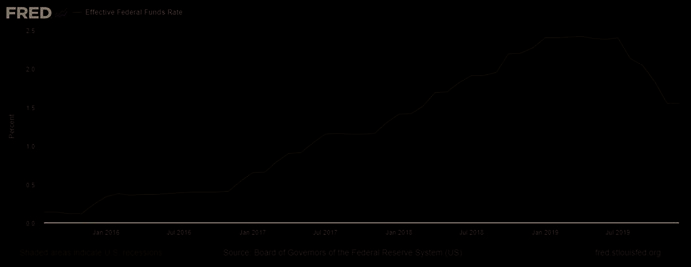
\includegraphics[width=0.8\textwidth]{gfx/m1l2_liq_exhibit3-1_fed_funds_rate.jpg}
    \caption{Lịch sử lãi suất Quỹ Liên bang (2015-2019)}
    \label{fig:fed_funds_rate}
\end{figure}

Dựa trên kỳ vọng của thị trường vào đầu tháng 10 năm 2018, những phát biểu của Chủ tịch Fed đã gây sốc cho hầu hết các nhà đầu tư. Họ lo sợ Fed có thể đang quá quyết liệt trong chính sách tiền tệ thắt chặt của mình và cuối cùng có thể đẩy nền kinh tế vào suy thoái. Do đó, lợi suất trái phiếu Kho bạc Hoa Kỳ kỳ hạn 10 năm (10-year U.S. Treasury note yields) ban đầu nhảy vọt lên 3,21\% sau thông báo, trước khi giảm xuống 2,69\% vào cuối năm 2018, trong khi chứng khoán sụt giảm 14\% trong suốt quý IV. Nỗi lo ngại về một cuộc suy thoái đã thúc đẩy những phản ứng mạnh mẽ này và tạo ra một mức độ biến động giá rất lớn trên thị trường trái phiếu và cổ phiếu. Hình 3.2 hiển thị lộ trình lợi suất trái phiếu Kho bạc trong năm 2018-2019, và Hình 3.3 hiển thị chỉ số thị trường chứng khoán S\&P 500 trong cùng khoảng thời gian này.

\begin{figure}[htbp]
    \centering
    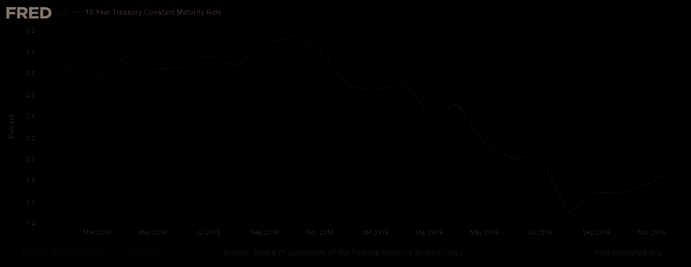
\includegraphics[width=0.8\textwidth]{gfx/m1l2_liq_exhibit3-2_treasury_yields.jpg}
    \caption{Lợi suất trái phiếu Kho bạc Hoa Kỳ kỳ hạn 10 năm (2018-2019)}
    \label{fig:treasury_yields}
\end{figure}

\begin{figure}[htbp]
    \centering
    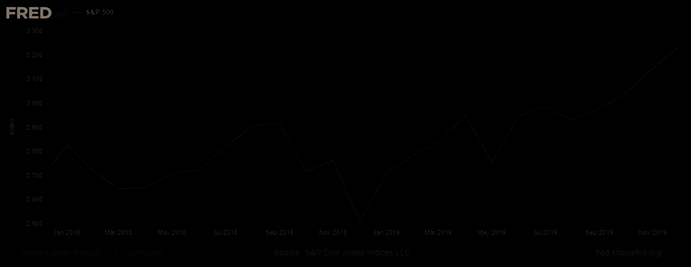
\includegraphics[width=0.8\textwidth]{gfx/m1l2_liq_exhibit3-3_sp500_longterm.jpg}
    \caption{Chỉ số thị trường chứng khoán S\&P 500 - Biến động dài hạn (2018-2019)}
    \label{fig:sp500_longterm}
\end{figure}

Hình 3.2 và 3.3 cung cấp những minh họa sống động về cách thức các thị trường tài chính tương tác với kinh tế vĩ mô theo hướng mà cả hai bên cùng ảnh hưởng lẫn nhau. Điều này có thể được nhìn thấy không chỉ ở sự sụt giảm nhanh chóng của lợi suất trái phiếu và giá cổ phiếu trong năm 2018, mà còn ở những phản ứng tích cực đối với các tuyên bố và hành động sau đó của Fed trong năm 2019, khi họ bắt đầu tạm dừng và cuối cùng là hạ lãi suất Quỹ Liên bang. Sau khi làm thị trường tài chính hoảng sợ ban đầu vào năm 2018, các hành động của Fed đã châm ngòi cho những đợt tăng điểm (rallies) lớn ở cả giá cổ phiếu và trái phiếu trong năm 2019.\footnote{Lưu ý rằng giá trái phiếu di chuyển ngược chiều với những thay đổi về lãi suất, do đó sự sụt giảm mạnh của lợi suất trái phiếu Kho bạc Hoa Kỳ kỳ hạn 10 năm từ mức hơn 3,2\% vào tháng 10 năm 2018 xuống còn 1,5\% vào tháng 8 năm 2019 đã tạo ra mức lợi nhuận vốn (capital gains) khổng lồ cho các nhà đầu tư trái phiếu.} Xuyên suốt quá trình này, các thành viên tham gia thị trường liên tục đánh giá bất kỳ thông tin mới nào về xu hướng của Fed, và bản thân Fed cũng theo dõi chặt chẽ các phản ứng của thị trường đối với những thay đổi trong chính sách tiền tệ của mình.

Chúng ta cũng có thể "phóng to" để kiểm tra xem thị trường chứng khoán đã phản ứng như thế nào với những bình luận của Chủ tịch Fed bằng cách nhìn vào các mức giá trong ngày (intraday prices) xung quanh những ngày diễn ra các tuyên bố này. Biến động giá trong ngày vào các ngày từ 3 đến 5 tháng 10 năm 2018 của chỉ số S\&P 500 được trình bày dưới đây.

\begin{figure}[htbp]
    \centering
    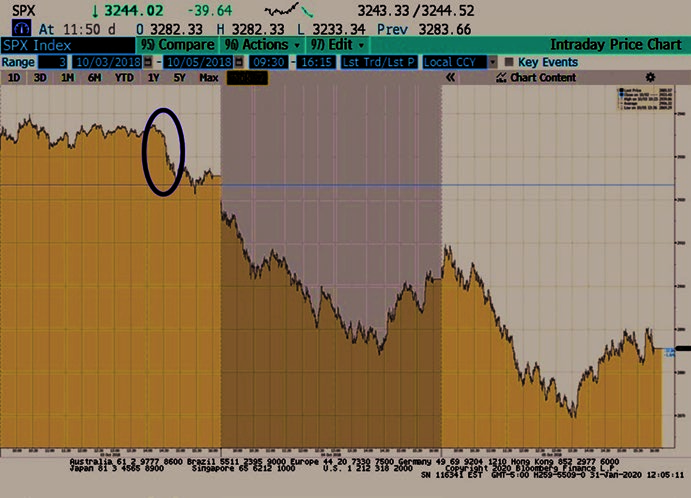
\includegraphics[width=0.8\textwidth]{gfx/m1l2_liq_exhibit3-4_sp500_intraday_oct3-5.jpg}
    \caption{Chỉ số thị trường chứng khoán S\&P 500 - Biến động trong ngày (3 tháng 10, 2018 - 5 tháng 10, 2018)}
    \label{fig:sp500_intraday_oct3-5}
\end{figure}

Như có thể thấy từ Hình 3.4, có một phản ứng mạnh mẽ và nhanh chóng đối với những bình luận bất ngờ của Chủ tịch Powell về việc cần phải tiếp tục tăng lãi suất. Cần lưu ý rằng phản ứng bắt đầu diễn ra vào buổi chiều ngày 3 tháng 10 ngay sau khi các bình luận của chủ tịch được công bố (được đánh dấu trong biểu đồ bằng hình bầu dục). Khi thị trường đạt được hiệu quả thông tin, chúng ta sẽ kỳ vọng loại phản ứng nhanh chóng này đối với các tin tức bất ngờ. Như được hiển thị dưới đây trong Hình 3.5 cho một ngày duy nhất, cú rơi ban đầu diễn ra ngay lập tức và rất dốc (giảm 0,4\% từ đỉnh của thị trường lúc 2:15 chiều cho đến khi đóng cửa lúc 4:00 chiều ngày 3 tháng 10); đợt bán tháo của thị trường tiếp diễn trong các ngày 4-5 tháng 10, tạo ra tổng mức giảm 1,8\% so với đỉnh trước thông báo\footnote{Nếu đợt sụt giảm trong hơn 2 ngày này được tính theo tỷ lệ hàng năm (annualized), khoản lỗ lũy kế sẽ xấp xỉ 84\% giá trị ban đầu của một nhà đầu tư sau 1 năm.}, do những thành viên tham gia thị trường lúc này đã xử lý đầy đủ các hệ lụy từ khả năng lãi suất tiếp tục tăng đối với nền kinh tế và các thị trường tài chính. 

\begin{figure}[htbp]
    \centering
    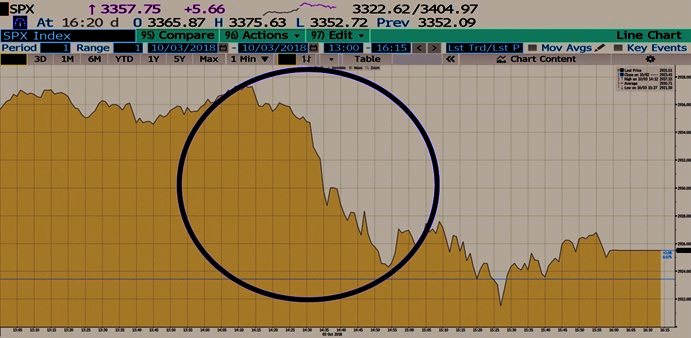
\includegraphics[width=0.8\textwidth]{gfx/m1l2_liq_exhibit3-5_sp500_intraday_oct3.jpg}
    \caption{Chỉ số thị trường chứng khoán S\&P 500 - Biến động trong ngày (3 tháng 10, 2018)}
    \label{fig:sp500_intraday_oct3}
\end{figure}

Bằng cách phóng to hơn nữa, chúng ta có thể thấy qua vòng tròn trong Hình 3.5 rằng phần lớn phản ứng ban đầu của chỉ số S\&P 500 xảy ra từ 2:15 chiều đến 2:55 chiều. Kiểu hình (pattern) này thường xuất hiện khi phản ứng ban đầu của thị trường tài chính là nhanh chóng và mạnh mẽ, nhưng như biểu đồ trước đó ở Hình 3.4 cho thấy, xu hướng giá có thể tiếp diễn trong nhiều ngày khi quá trình hài hòa giữa các kỳ vọng phân kỳ thông qua giao dịch giữa "phe bò" (bulls) và "phe gấu" (bears) dần được bộc lộ.

Trái ngược với hành vi của thị trường chứng khoán vào tháng 10 năm 2018 được hiển thị ở trên, chúng ta cũng có thể xem xét một phản ứng mạnh và nhanh khác, nhưng lần này là theo chiều ngược lại của chỉ số S\&P 500. Như đã lưu ý trước đó, thị trường phản ứng tích cực với các bình luận ôn hòa hơn của Powell liên quan đến việc tạm dừng các đợt tăng lãi suất tiềm năng trong tương lai vào đầu năm 2019. Phản ứng này có thể được nhìn thấy trong Hình 3.6 thông qua các mô hình giá trong ngày đối với chỉ số chứng khoán chính yếu này trong hai ngày 3-4 tháng 1 năm 2019.

\begin{figure}[htbp]
    \centering
    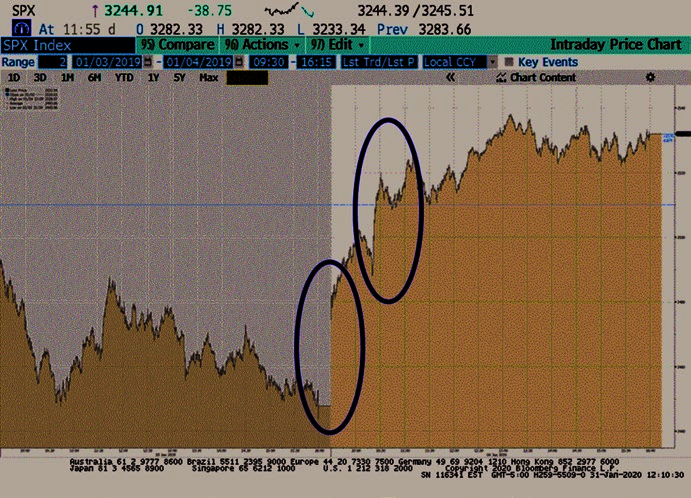
\includegraphics[width=0.8\textwidth]{gfx/m1l2_liq_exhibit3-6_sp500_intraday_jan3-4.jpg}
    \caption{Chỉ số thị trường chứng khoán S\&P 500 - Biến động trong ngày (3 tháng 1, 2019 - 4 tháng 1, 2019)}
    \label{fig:sp500_intraday_jan3-4}
\end{figure}

Hình 3.6 cho thấy một cú nhảy vọt lớn vào sáng sớm ngày 4 tháng 1 năm 2019 (xem hình bầu dục đầu tiên trên biểu đồ). Phản ứng tích cực ban đầu khi thị trường mở cửa lúc 9:30 sáng là do một báo cáo về việc làm phi nông nghiệp (nonfarm employment report) mạnh mẽ một cách đáng ngạc nhiên được công bố sớm hơn vào sáng hôm đó lúc 8:30 sáng, cho thấy 312.000 việc làm đã được tạo ra ở Hoa Kỳ trong tháng 12 năm 2018. Ngay khi thị trường chứng khoán mở cửa trở lại lúc 9:30 sáng ngày 4 tháng 1, chỉ số chứng khoán S\&P 500 đã tăng vọt lên 2.475,90 (mức tăng 1,1\% so với mức đóng cửa của ngày hôm trước là 2.447,89). Cú nhảy lớn và không liên tục này từ mức giá đóng cửa trước đó được gọi là "gap up" (tạo khoảng trống giá lên) trong ngôn ngữ của phân tích kỹ thuật. Đây là một ví dụ kinh điển về cách các thị trường tài chính phản ứng nhanh chóng với những tin tức tích cực bất ngờ về kinh tế vĩ mô.

Thị trường chứng khoán sau đó đã nhảy vọt lần thứ hai vào cuối buổi sáng hôm đó, giữa 10:00 sáng và 11:00 sáng, do Chủ tịch Powell tuyên bố rằng Fed đang cân nhắc việc tạm dừng các đợt tăng lãi suất Quỹ Liên bang trong tương lai. Giống như mô hình (pattern) được hiển thị trước đó trong Hình 3.4 và 3.5, các bình luận công khai của Chủ tịch về chính sách tiền tệ là nằm ngoài dự đoán, và do đó, các nhà giao dịch và nhà đầu tư đã phản ứng nhanh chóng, như có thể thấy ở hình bầu dục thứ hai trên Hình 3.6. Hiệu ứng ròng (net effect) đối với giá cổ phiếu là cực kỳ nhanh và lớn. Sau đó, chỉ số này tiếp tục xu hướng đi lên trong phần còn lại của ngày và đóng cửa ở mức 2.531,94, tạo ra mức lợi nhuận tổng cộng 3,02\% so với mức đóng cửa của ngày hôm trước. Đây là một mức tăng rất lớn vì các chỉ số thị trường chứng khoán của Hoa Kỳ thông thường biến động dưới 1\% mỗi ngày.

Hình 3.7 cho thấy sự khác biệt về thanh khoản của các chứng khoán cá nhân có thể ảnh hưởng đến quá trình khám phá giá như thế nào xung quanh các bình luận của Chủ tịch Powell vào ngày 4 tháng 1 năm 2019. Để minh họa hai cổ phiếu có thể phản ứng theo những cách rất khác nhau đối với cùng một tin tức từ Chủ tịch Fed, Hình 3.7 hiển thị các mô hình giá trong ngày từ 9:30 sáng đến 11:15 sáng hôm đó đối với một cổ phiếu có tính thanh khoản rất cao là Microsoft (một gã khổng lồ phần mềm toàn cầu), và một cổ phiếu có tính thanh khoản khá kém là Flushing Financial (một ngân hàng thương mại nhỏ có trụ sở tại Thành phố New York). Đường màu trắng trích xuất những biến động của cổ phiếu Microsoft, trong khi đường đứt nét biểu thị các chuyển động của Flushing Financial.\footnote{Cả hai cổ phiếu đều đã được lập chỉ mục (indexed) đến giá trị cơ sở ban đầu là 100 để dễ so sánh.} Có thể nhận thấy rằng mô hình giá của Microsoft trơn tru hơn rất nhiều vì các giao dịch xảy ra thường xuyên và ở các mức giá khá gần với các mức giá trước đó. Do vậy, bất chấp tin tức lớn từ Fed trong ngày hôm đó, cổ phiếu của Microsoft vẫn phản ứng nhanh chóng và theo một cách "công bằng và có trật tự" vì nhiều giao dịch đã được thực hiện liên tục trong từng phút giao dịch.

\begin{figure}[htbp]
    \centering
    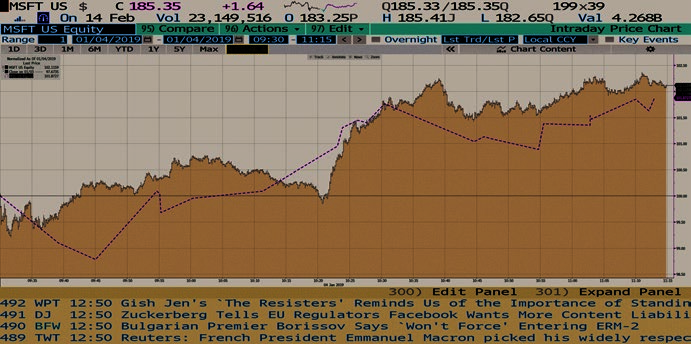
\includegraphics[width=0.8\textwidth]{gfx/m1l2_liq_exhibit3-7_large_vs_small_cap.jpg}
    \caption{Biến động trong ngày của Cổ phiếu vốn hóa lớn so với Cổ phiếu vốn hóa nhỏ (4 tháng 1, 2019)}
    \label{fig:large_vs_small_cap}
\end{figure}

Trái ngược lại, đường đứt nét của Flushing Financial di chuyển theo một cách thức đột ngột và lởm chởm vì cổ phiếu của nó không giao dịch thường xuyên đến vậy. Điều này cũng dẫn đến việc giá cổ phiếu bị tụt hậu (lag) so với những biến động của chỉ số thị trường chứng khoán S\&P 500 và của Microsoft. Trên thực tế, trong khoảng thời gian 9:30-11:15 sáng của ngày hôm đó, cổ phiếu Flushing Financial chỉ giao dịch vỏn vẹn 25 lần, trong khi Microsoft được giao dịch tới 2.520 lần! Hơn nữa, tổng khối lượng giao dịch cổ phiếu hàng ngày (daily share trading volume) đối với Microsoft là 44.061.000, và đối với Flushing Financial chỉ là 67.250.

Điều này thể hiện một sự khác biệt rất lớn về hoạt động giao dịch, trong đó cổ phiếu của Microsoft có tính thanh khoản cao hơn hẳn, do người mua và người bán có thể dễ dàng giao dịch vào bất kỳ thời điểm nào trong phiên giao dịch (ví dụ: trung bình 24 lần mỗi phút). Ngược lại, cổ phiếu của Flushing Financial không giao dịch quá thường xuyên trong khoảng thời gian này (một lần mỗi 4,2 phút), và do đó, giá của nó buộc phải dịch chuyển mạnh hơn vào thời điểm nó thực sự có giao dịch nhằm "bắt kịp" với các tin tức về báo cáo việc làm của Hoa Kỳ và các bình luận của Chủ tịch Fed. Do đó, việc khám phá ra mức giá "chính xác" đối với một cổ phiếu kém thanh khoản như Flushing Financial khó khăn hơn rất nhiều vì thiếu các giao dịch thường xuyên. Mặc dù biểu đồ này chỉ cho thấy hai cổ phiếu, những sự khác biệt về thanh khoản như vậy tồn tại ở hàng nghìn cổ phiếu được giao dịch tại Hoa Kỳ trong bất kỳ ngày nào.

Cơ chế giao dịch và quá trình khám phá giá được mô tả trước đó trong chương này là những công cụ thiết yếu cần có nhằm tạo thuận lợi cho những tương tác này giữa kinh tế vĩ mô và thị trường tài chính. Do vậy, việc sở hữu những thị trường tài chính hoạt động tốt và có tính thanh khoản cao là vô cùng quan trọng, giúp các tín hiệu giữa các nhà hoạch định chính sách, nhà đầu tư, giám đốc kinh doanh và người tiêu dùng trở nên rõ ràng nhất có thể.

